\documentclass{article}
\usepackage{style}
\usepackage[utf8]{inputenc}
\usepackage{placeins}
\usepackage{booktabs} 
\usepackage{longtable}
\usepackage[title]{appendix}
\usepackage{amssymb}

\graphicspath{{media/}}

\title[Primality Testing]{Probablistic Primality Testing and Analysis of Probablistic AKS}
\author[Emilie Ma]{%
Emilie Ma\\%
University of British Columbia\\%
\texttt{kewbish@gmail.com}%
}
\date{\today}
\mentor{Pressiana Marinova\\%
Occado Technology Sofia\\%
\texttt{pressiana.marinova@gmail.com}%
}

\begin{document}
\maketitle
\newpage
\begin{abstract}
    This paper aims to analyze the Fermat, the Euler (Solovay-Strassen), and the Miller-Rabin primality tests, three well-known probabilistic algorithms based on Fermat's little theorem. The Agarwal-Kayal-Saxena test, the first polynomial time deterministic primality test developed, is also discussed, as well as a proposal for a new probabilistic adaptation.
\end{abstract}

\section{Introduction}
Prime numbers, or numbers with no factors other than 1 and itself, are of crucial importance in cryptography and cybersecurity. Many encryption algorithms, such as the frequently used Rivest-Shamir-Adleman (RSA) cryptosystem, rely on the 'trapdoor' nature of prime numbers: while multiplying prime numbers is trivial, finding the factors of a composite number is computationally expensive. 
Since cryptography is so widely applied, generating prime numbers for use in encryption cryptosystems is a major issue and field of research.

There is no known pattern to identify prime numbers, so to generate a prime number, a random number $n$ is first generated. This number $n$ is then passed through a primality test, or an algorithm designed to identify if a number is prime or not. A variety of algorithms may be used, including the Fermat, Euler or Solovay-Strassen, Miller-Rabin, and Agarwal-Kayal-Saxena (AKS) tests.

These tests, except the AKS test, are \emph{probabilistic}. A probabilistic test is an algorithm that utilizes some form of randomness in its design; for example, random trial bases may be selected from a range of possibilities. In contrast, a deterministic algorithm, when given an input, will always return the same output. Minimizing the running time of primality tests is desired to increase the efficiency of generating random primes, so often, probabilistic tests are used due to their shorter running time and increased practicality. However, probabilistic tests have a small probability of designating a number as prime when it is composite. This is avoided with deterministic primality tests, such as the AKS test discussed in section \ref{theory:aks}, but issues with impractical running times arise.

The AKS test is notable for being the first polynomial time deterministic primality test. Polynomial time refers to a concept of Big-O theory, or the notation that describes the upper bound of a function when its input tends towards infinity. In Big-O notation, polynomial time, or a function of form $O(n^x)$ is preferred to a function of form $O(x^n)$ for some input size $n$ and value $x$, as $x^n$ will grow faster than $n^x$ as $n$ increases. In other words, $n^x$ algorithms remain more efficient than $x^n$ ones in worst-case scenarios. 

However, even though AKS is bounded by a polynomial time, it remains impractical and incredibly slow compared to other probabilistic tests. As Richard Brent showed in a 2010 comparison with the Miller-Rabin and other probabilistic primality tests found that where 100 trials of Miller-Rabin took 0.3 seconds to process, AKS would take an estimated 37 weeks to run one trial on the same number (equivalent, as AKS is deterministic and only requires one run to determine the output). These times are unfeasible for applied usage, so research into optimizing and discovering probabilistic tests remains relevant.
% TODO: https://maths-people.anu.edu.au/~brent/pd/comp4600_primality.pdf
% TODO: https://ieeexplore.ieee.org/document/7942510
% TODO: http://depts.washington.edu/uwmxl/wordpress/wp-content/uploads/2017/05/AKS_Final_Report.pdf

As an alternative, this paper proposes a probabilistic version of AKS, inspired by methods used by the Fermat, Euler (Solovay-Strassen), and Miller-Rabin tests in choosing a range of random numbers to test against certain congruences and theorems.

\section{Background Number Theory}

Many probabilistic primality tests rely on number theory and modular arithmetic to test for primality. The Fermat, Euler (Solovay-Strassen), Miller-Rabin, and AKS tests and their background theory are discussed below.

Note that all $\log{n}$ in this paper are assumed to be taken as $\log{2}{n}$ unless otherwise marked.

\subsection{Fermat Primality Test}
The Fermat Primality Test is a probabilistic primality test based on Fermat's little theorem.
Fermat's little theorem, developed by Pierre de Fermat in 1640, states that for any integer $a$ and any prime $p$, the following holds:
\[
    a^p \equiv a \pmod{p} 
\]
If $a$ is not divisible by, or \emph{coprime} to, p, the following is equivalent:
\[
    a^{(p - 1)} \equiv 1 \pmod{p} 
\]

\begin{proof} % https://artofproblemsolving.com/wiki/index.php/Fermat%27s_Little_Theorem
Consider $S = \{a, 2a, 3a, \ldots{}, (p - 1) * a\}$.
Suppose $ra$ and $sa$ in the set are equal $\pmod{p}$, so $r \equiv s \pmod{p}$.
Therefore, the $p - 1$ multiples of $a$ in $S$ are uniquely distinct, and must be congruent to ${1, 2, 3, \ldots{}, (p - 1)}$ in some order.
Multiply these congruences like so:
    \[a * 2a * 3a * \ldots{} * (p - 1)a \equiv 1 * 2 * 3 * \ldots{} (p - 1) \pmod{p}\]
This gives:
    \[a^{(p - 1)} * (p - 1)! \equiv (p - 1)! \pmod{p}\]
Divide by $(p - 1)!$ on each side for:
    \[a^{(p - 1)} \equiv 1 \pmod{p}\]
To arrive at the alternate form of Fermat's Little Theorem, multiply both sides by $a$.
    \[a^p \equiv a \pmod{p}\]
\end{proof}

Knowing that $a^{(n - 1)} \equiv 1 \pmod{n}$ holds if $n$ is prime, Fermat's primality test chooses $k$ random integers $a$ coprime to $n$ to test if all $a$ are congruent to 1. Because this holds trivially for $a \equiv 1 \pmod{n}$ and if $n$ is odd and $a \equiv -1 \pmod{n}$, $a$ is conventionally chosen such that $1 < a < n - 1$. Higher values of $k$ indicate a higher probability that the number is prime.

If $n$ passes these $k$ base tests, it is known as a probable prime. However, not all numbers that pass the Fermat primality test are prime - composite numbers $n$ that pass the test are known as Fermat pseudoprimes. There are infinitely many Fermat pseudoprimes, and several forms of composite numbers that pass the test. For example, Carmichael numbers, composite numbers that satisfy the relation $b^{(n-1)} \equiv 1 \pmod{n}$ for all integers $b$ coprime to $n$, all pass Fermat's primality test.

\subsection{Euler (Solovay-Strassen) Test} % https://artofproblemsolving.com/wiki/index.php/Euler%27s_Totient_Theorem
The Solovay-Strassen Test is another probabilistic test, utilizing the properties of Euler's theorem. Proposed by Leonhard Euler in 1763, Euler's theorem is a generalization of Fermat's little theorem, stating that if $a$ and $p$ are coprime, then the following holds:
\[
    a^{\phi(n)} \equiv 1 \pmod{n}
\]
The function $\phi(n)$ is Euler's totient function. The totient of some number $n$ is the number of positive integers $l$ in the range $1 <= l <= n$ where l is coprime to n.

\begin{proof}
    Consider $S = \{1 <= l <= n | gcd(l, n) = 1\} = \{l_1, l_2, l_3, \ldots{}, l_{\phi(n)}\}$.
    Create a set $aS = \{al_1, al_2, al_3, \ldots{}, al_{\phi(n)}\}$. \\
    All elements of $aS$ are relatively prime to $n$, so if all elements of $aS$ are distinct, $aS = S$. All elements of $aS$ are distinct, as all elements of $S$ are distinct. Therefore, each element of $aS \equiv S \pmod{n}$.
    Therefore:
    \[
        l_1 * l_2 * l_3 * \ldots{} * l_{\phi(n)} \equiv al_1 * al_2 * al_3 * \ldots{} * al_{\phi(n)} \pmod{n}
    \]
    As $l_1 * l_2 * l_3 * \ldots{} * l_{\phi(n)}$ is relatively prime to $n$, reducing this gives:
    \[
        a^{\phi(n)} * l_1 * l_2 * l_3 * \ldots{} * l_{\phi(n)} \equiv l_1 * l_2 * l_3 * \ldots{} * l_{\phi(n)} \pmod{n}
    \]
    Therefore, $a^{\phi(n)} \equiv 1 \pmod{n}$.
\end{proof}

Fermat's little theorem is considered a special case of Euler's theorem, because if $n$ is prime, $\phi(n) = n - 1$.

Given that $a^{\phi(n)} \equiv 1 \pmod{n}$, then 
\[
    a^{\phi(n) / 2} \equiv \begin{cases}
\;\;\,1\pmod{n}& \text{ when there exists }x \text{ such that }a\equiv x^2 \pmod{n}\\
     -1\pmod{n}& \text{ when there is no such integer.}
\end{cases}
\]

The conditions above form the criteria for the Legendre symbol of $a$ and $n$. The Legendre symbol $(\frac{a}{n})$ is defined like so:
\[
    (\frac{a}{n}) \begin{cases}
        0 & \text{ when $a \equiv 0 \pmod{n}$} \\
        -1& \text{ when $a \not\equiv 0 \pmod{n}$ and there exists $x: a \equiv x^2 \pmod{n}$} \\
     -1& \text{ when $a \not\equiv 0 \pmod{n}$ and there is no such integer $x$.}
\end{cases}
\]

The Jacobi symbol is the generalization of the Legendre symbol to any odd integer $n$, and is used in the Solovay-Strassen primality test. It is defined as the product of the Legendre symbols of $n$'s prime factors, such that:
\[
    (\frac{a}{n}) = (\frac{a}{p_1})^{\alpha_{1}} * (\frac{a}{p_2})^{\alpha_{2}} * \ldots{} * (\frac{a}{p_k})^{\alpha_{k}}
\]
for $n = p_1^{\alpha_{1}} * p_2^{\alpha_{2}} * \ldots{} * p_k^{\alpha_{k}}$.

As with Fermat's primality test, $k$ random bases $a$ are tested. If $a^{(n - 1) / 2} \equiv (\frac{a}{n}) \pmod{n}$ holds for all $k$ basis, then $n$ is a probable prime.

Similar to Fermat's primality test, the Solovay-Strassen test may pass composite numbers as primes. These are then known as Euler (sometimes Euler-Jacobi) pseudoprimes or liars. All Euler pseudoprimes are also Fermat pseudoprimes. 

\subsection{Miller-Rabin Primality Test} % http://home.sandiego.edu/~dhoffoss/teaching/cryptography/10-Rabin-Miller.pdf
A third probabilistic primality test, the Miller-Rabin primality test was developed first by Gary Miller in 1976, and subsequently modified by Michael Rabin in 1980. The test relies on two congruence relations that hold when $n$ is an odd prime and rewritten as $2^s * d + 1$, and $a$ is a base such that $0 < a < n$:
\begin{gather*}
    a^d \equiv 1 \pmod{n} \\
    a^{(2^r * d)} \equiv -1 \text{ for some $r$ such that $0 <= r < s$}
\end{gather*}

Because $n$ is written as $2^s * d + 1$, $n - 1 = 2^s * d$. Therefore, if $a^d \equiv \pm 1 \pmod{n}$, then $n$ is a strong probable prime.

\begin{proof}
    Given that:
    \[
        a^{(n - 1)} \equiv (a^d)^{2^s} \equiv 1 \pmod{n}
    \]
    for all prime $n$, and because there are no square roots of 1 other than $\pm 1$, the repeated squaring with $2^s$ doesn't affect the congruence.
\end{proof}

Otherwise, $a^d \pmod{n}$ is squared, for $a^2d$. If $a^2d \equiv 1 \pmod{n}$, n is composite, because there are different square roots of $a^2m \pmod{n}$ other than $\pm 1$. If $a^2d \equiv -1 \pmod{n}$, then $n$ is a probable prime for similar reasons as above.

These checks are repeated until $a^{(2^{(s - 1)} * d)}$ has been reached. If it is $\pm 1$, the result is known by the tests above; however, if not, $n$ is composite, by Fermat's little theorem.

\subsection{Agarwal-Kayal-Saxena (AKS) Primality Test} % https://www.cse.iitk.ac.in/users/manindra/algebra/primality_v6.pdf
\label{theory:aks}
By contrast, the AKS primality test is a deterministic primality test first proprosed by Manindra Agarwal, Neeraj Kayal, and Nitin Saxena in 2002. It is the first primality test to deterministically verify primality in polynomial time for all number inputs, with a time complexity bound of $\mathcal{O}(\log{(n)}^{21/2})$.

The test is based on the theorem that an integer $n >= 2$ and an integer $a$ coprime to $n$, $n$ is prime if and only if the below holds within the polynomial ring $\mathbb{Z}[x]$, or the ring of polynomials with degree at most $n$ over $\mathbb{Z}$.
\[
    (X + a)^n \equiv X^n + a \pmod{n}
\]

\begin{proof} % http://www.cs.tau.ac.il/~amnon/Classes/2019-Derandomization/Lectures/Lecture7-AKS-All.pdf
    This is a generalization of Fermat's little theorem over polynomials, proven with the binomial identity.
    \[
        (x + a)^n = \sum_{i=0}^{n} \binom{n}{i} x^i a^{n - i} where \binom{n}{0} = \binom{n}{n} = 1
    \]
    If $n$ is prime, then:
    \[
        \binom{n}{i} = \frac{n (n - 1) \ldots{} {n - i + 1}}{i!}
    \]
    for all i > 1. When taken $\pmod{n}$, $n$ divides the numerator once; therefore, $\binom{n}{i} \equiv 0 \pmod{n}$. $a$ does not necessarily need to be coprime with $n$.
    If $n$ is not prime, and $a$ is coprime with $n$, then $n$ has a prime factor of form $p^k$. $p^k$ will divide $n$, but $p^{k - 1}$ will not. Given the monomial with a coefficient of:
    \[
        \binom{n}{i} = \frac{n (n - 1) \ldots{} {n - p + 1}}{p!}
    \]
    $p^k$ divides $n$, but not $(n - 1) \ldots{} (n - p + 1)$. Therefore, $p^k \vert n (n - 1) \ldots{} (n - p + 1)$ but $p^{k + 1} \nmid n (n - 1) \ldots{} (n - p + 1)$. $p$ also divdes $p$, but not $1 \ldots p$, so $p \vert p!$ but $p^2 \nmid p!$. This gives $p^{k - 1} \vert \binom{n}{p}$ and $p^k \nmid \binom{n}{p}$. As $p^k$ is a factor of $n$, $n \nmid \binom{n}{p}$, and $x^p$ does not vanish.
\end{proof}

The test begins by ensuring $n$ is not a perfect power, or a number of form $a^k$ for some $a$ and $k$. If it is, the number is composite.

Next, the algorithm finds the smallest $r$ such that $ord_r(n) > {\log{n}}^2$ and $r$ is coprime to $n$.

The algorithm then checks for all $2 <= a <= min(r, n - 1)$ that $a \nmid n$. If $a \vert n$ for some $a$ in this range, the number is composite. This is equivalent to trial division up to $r$.

If $n <= r$, the number is prime, as this is equivalent to trial division to $\sqrt{n}$.

The last step of the algorithm reduces the time complexity from exponential to polynomial time by operating over the finite ring $(\mathbb{Z}/(n))[X] / (X^r - 1)$. Each $a$ from $1 <= a <= \lfloor \sqrt{\varphi(r)}\log_2(n) \rfloor$ is checked for the generalized Fermat's theorem. If it does not pass, the number if composite; if it passes, the number is prime.

\section{Running Time}
This section discusses the running time bounds of the tests with Big-O notation.

In Big-O notation, $\widetilde{O}(f(n))$ is a shorthand for $O(f(n) * log{f(n)}^k)$ for some $k$, ignoring the logarithm factor due to the growth effects of other operations in $f(n)$.

\subsection{Fermat Primality Test}
The Fermat primality test implementation tested used repeated squaring and multiplication techniques, requiring several modular computations per bit of each number $n$ tested. The number of bits in $n$ is $\log{n}$, so as there are $k$ iterations of a modular exponentiation applied, the final complexity is $O(k * log{n})$.

\subsection{Euler (Solovay-Strassen) Primality Test}
The Euler (Solovay-Strassen) primality test is implemented in three main steps: the coprime to $n$ check, the computation of the Jacobi symbol $(\frac{a}{n})$, and the modular exponentiation.Checking if a number is coprime to another involves a greatest-common-denominator test, which can be run in a time of $O(log{n})$ where $log{n}$ is again the size of the number in bits. Similarly, the Jacobi symbol and modular exponential can both also be run in $O(log{n})$ time, so the final complexity is:
\[
    O(k * log{n} * log{n} * log{n}) = O(k * log^3{n})
\]

\subsection{Miller-Rabin Primality Test}
Similar to the Euler (Solovay-Strassen) test, the Miller-Rabin test runs in $O(k * log^3{n})$ time, due again to the modular exponentiation operations.

\subsection{AKS Primality Test}
The AKS paper originally detailed the time complexity of the algorithm as $\widetilde{O}(log(n)^{12})$ with the use of fast modular exponentiation techniques (like repeated squaring). However, the paper was later revised to give the time complexity $\widetilde{O}(log(n)^{15/2})$ based on new proofs.

In 2005, after Pomerance and Lenstra developed an AKS variant with a running time of $\widetilde{O}(log(n)^{6})$, the paper was again updated.

\section{Probabilistic AKS}

\subsection{Effects on Pseudoprimes}

\subsection{Running Time}

\section{Methods}
The primality tests were subject to a similar analysis method over multiple trials; the raw data is available in Appendix \ref{appendix:data}. For the probablistic tests, each trial tested a different $k$ value, and consisted of:

\begin{itemize}
    \item{Generating a random set ($S$) of $10^4$ odd integers such that $10^5 < x < 10^6$. This interval was chosen due to an intersection of higher concentrations of pseudoprimes found for meaningful data comparisons between each trial and reasonable running times for the trials conducted.}
    \item{Using Sympy's \texttt{is\_prime} (which runs a variant of the Baillie-Pomerance-Selfridge-Wagstaff probablistic primality test) to check for primality for each integer in $S$}
    \item{Running the primality test with $k$ attempts run on each integer in $S$ with respect to some base $a$}
    \item{Counting all pseudoprimes which passed the primality test but not Sympy's primality test}
    \item{Return lowest number of bases tried (lowest $k$) that returned the lowest number of pseudoprimes passed, the maximum and minimum number of pseudoprimes, and the average pseudoprimes found}
\end{itemize}

Each trial was timed with the Python \texttt{timeit} command, recording the total wall time elapsed. Data for average time taken per $k$ value was collected in a similar way. 

For the Fermat, Euler (Solovay-Strassen), and Miller-Rabin tests, the results of fifty trials were recorded, ranging from $k = 1$ to $k = 100$.

Note that for deterministic AKS, the testing method consisted of running a single trial over a random set $S$, within the same bounds, but with $10^3$ integers tested, for practicality reasons. A trial of $10^4$ random integers at that range took around 118 min, and fifty trials would have been impractical for the scope of this inquiry.

For probablistic AKS, the testing method consisted of running fifty trials over the random set $S$. However, $k$ only ranges from $1 <= k <= 5$, again for practical reasons. During analysis, a trial of the first $10^4$ integers with $k = 50$ took over \iffalse TODO: add time \fi min.

The raw data of each of the primality tests can be found in Appendix \ref{appendix:data}.
See Appendix \ref{appendix:tech} for primality test implementation details and hardware specifications.

\section{Results}
For the Fermat, Euler (Solovay-Strassen), and Miller-Rabin tests, the results of trials ranging from $k = 1$ to $k = 50$ are shown. For $k$ values greater than 50, it was found that pseudoprimes were found very rarely (around 5 pseudoprimes found in total over 50 trials of $50 <= k <= 100$) across all three tests. Additional base analysis data can be found in Appendix \ref{appendix:data}.

In Figure \ref{fig:pprimes_v_bases}, the average number of pseudoprimes passed per $k$ bases tested is shown. All test exhibit a similar pattern of passing larger number of pseudoprimes with lower amounts of bases tested $k$. The Fermat primality test passed the most pseudoprimes, with an average of 6.5 pseudoprimes at $k = 1$. The Euler (Solovay-Strassen) test passed an average of 3.2 pseudoprimes at $k = 1$, while the Miller-Rabin test passed a similar average of 3.3. The Fermat primality test has low ($<0.1$) average numbers of pseudoprimes passed beginning around $k = 25$. The Euler test passes low numbers of pseudoprimes at around $k = 5$, and at $k = 3$, the Miller-Rabin test begins to pass low numbers of pseudoprimes. Both the Euler and Miller-Rabin tests pass consistent averages of 0 pseudoprimes after their respective drop-off points; however, the Fermat test wavers around 0 to 0.1 pseudoprimes passed for all trials after $k = 25$.

Figure \ref{fig:time_v_bases} shows the time elapsed for $k$ base trials over $k$ bases tested.

\FloatBarrier
\begin{figure}[h!]
\label{fig:pprimes_v_bases}
\caption{The effect of increasing the number of base trials $k$ on pseudoprimes passed}
\centering
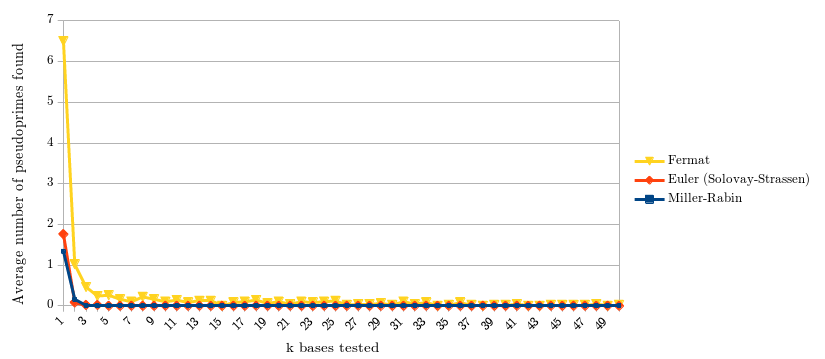
\includegraphics[width=0.8\textwidth]{pprimes_v_bases}
\end{figure}
\FloatBarrier

\FloatBarrier
\begin{figure}[h!]
\label{fig:time_v_bases}
\caption{The effect of increasing the number of base trials $k$ on running time elapsed}
\centering
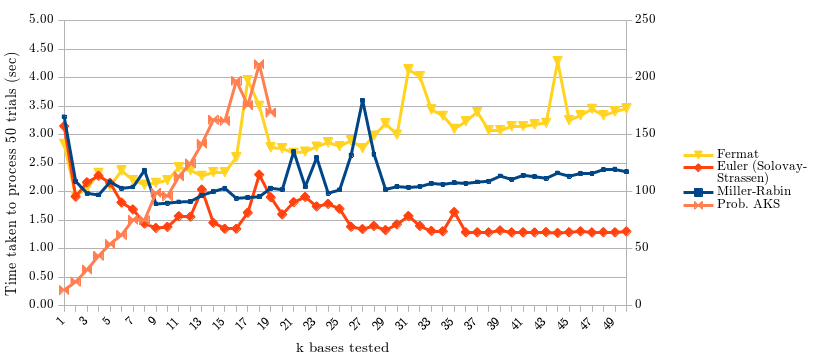
\includegraphics[width=0.8\textwidth]{time_v_bases}
\end{figure}
\FloatBarrier

\FloatBarrier
\begin{figure}[h!]
\label{fig:pprimes_v_trial}
\caption{Average pseudoprimes passed across all $1 <= k <= 50$ values per trial}
\centering
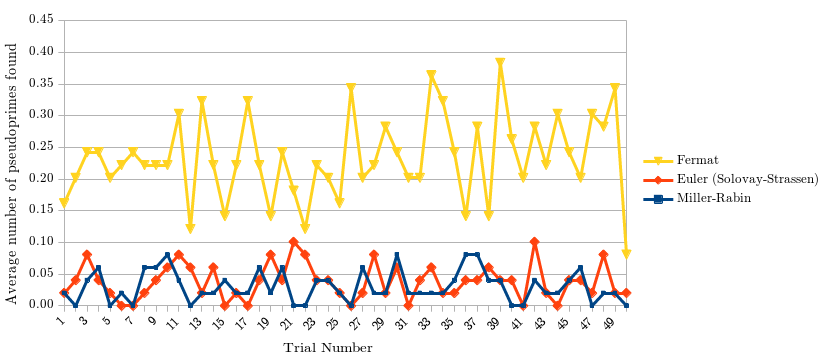
\includegraphics[width=0.8\textwidth]{pprimes_v_trial}
\end{figure}
\FloatBarrier

\FloatBarrier
\begin{figure}[h!]
\label{fig:time_v_trial}
\caption{Running time elapsed across all $1 <= k <= 50$ values per trial}
\centering
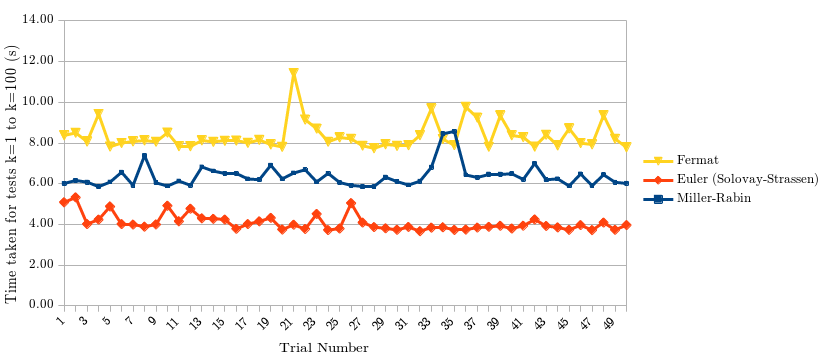
\includegraphics[width=0.8\textwidth]{time_v_trial}
\end{figure}
\FloatBarrier

% TODO: det AKS vs prob AKS

\section{Discussion}
Note that as the determinism of AKS under the small interval used for testing has already been proven, the . Trials run on 

\subsection{Sources of Error}
A possible source of error present includes the range of numbers tested for pseudoprimes and the distribution of pseudoprimes over said range. % TODO: https://cr.yp.to/bib/1980/pomerance-pseudo.pdf
As Pomerance, Selfridge, and Wagstaff showed in their 1980 analysis on pseudoprimes to $25 * 10^9$, there are 167 Fermat pseudoprimes, 78 Euler psuedoprimes, and 30 strong (Miller-Rabin) pseudoprimes between $10^5$ and $10^6$. In larger intervals between larger numbers, the amount of these pseudoprimes grows. However, with larger intervals, the probability of randomly selecting pseudoprimes within $10^4$ choices decreases. Increasing the bounds of the tests was outside the scope of this examination, but may be left to future research. Running the primality tests over a larger interval of larger numbers with a higher amount of choices may improve this analysis. 

\section{Conclusion}
Conclusion + propose further inquiry

\nocite{*}
\bibliographystyle{plainnat}
\bibliography{references}

\appendix
\begin{appendices}
\section{Raw Data for Primality Tests} \label{appendix:data}

The raw data for each of the primality tests can be found \href{https://github.com/kewbish/srs/tree/master/scripts/dataset}{here}. % TODO: Ensure correct link if I restructure files
The data is available in CSV format, labelled by primality test (Fermat, Euler, Miller-Rabin, deterministic AKS, and probablistic AKS). The folder also includes other data not discussed in-depth in this paper, including several base analysis types (all bases generated randomly, base 2, base 3, base 5, or a combination of bases 2 and 3, bases 3 and 5, and bases 2 and 3).

Each row in the CSV file is a trial of the given test with given base. The first hundred columns represent the pseudoprimes found at $k$ trials of different bases. The last four columns represent the average pseudoprimes found over the entire trial from $1 <= k <= 100$, the lowest $k$ value required to pass the lowest number of pseudoprimes, the lowest number of pseudoprimes, and the time required to run the test in minutes and seconds. 
The last row, which contains only 50 values, should be interpreted as the average time taken for a trial of $k$ bases, where $k$ is the column number.

\section{Technical Details} \label{appendix:tech}

\subsection{Primality Test Implementations}
The implementations of the primality tests can be found on GitHub at kewbish/srs. % TODO: citation on GitHub
The tests were implemented with Python 3.7, with the Numpy and Numba libraries used to optimize computations, and the Sympy library used to test for primality.
The AKS primality test implementation was iterated on from a reference implementation by Sophoclis Stephanou was found on GitHub. % TODO: citation

\subsection{Hardware}
The primality tests ran on a HP-15bs028ca running Manjaro Linux x86\_64 and kernel 5.10.49-1-MANJARO, with a 4-core Intel i5-7200U (4) 3.100GHz CPU and 16.0GiB of RAM.

\end{appendices}

\end{document}

